%
%  愛知工業大学 情報科学部 情報科学科
%    要旨集用LaTeXテンプレート(2016.11.28)
%
%  original by Nobuhiro Ito
%  revised by Susumu Suzuki & Masashi Morimoto on 2016.11.28
%
\documentclass{jarticle}
\pagestyle{empty}

%% レイアウト
\setlength{\topmargin}{-10.4mm}
\setlength{\headheight}{0mm}
\setlength{\headsep}{0mm}
\setlength{\textheight}{262mm}
\setlength{\textwidth}{180mm}
%\setlength{\topskip}{7mm}
\setlength{\evensidemargin}{-10.4mm} 
\setlength{\oddsidemargin}{-10.4mm} 
\setlength{\columnsep}{8mm}

%% パッケージ環境
% graphicx: 画像読み込み
%  dvipdfmxをドライバ指定することでpdf/png/jpeg形式の図を利用可能
%  異なるドライバを利用する場合はそのドライバ指定に変更
% \usepackage{graphicx} % suzuki
\usepackage[dvipdfmx]{graphicx} % suzuki
% subcaption: subfigureを置き換えたパッケージ(複数の図用)
% \setlength{\footskip}{12mm}
% \usepackage{subfigure}	 % suzuki
\usepackage{subcaption} % suzuki
% color:文章に色をつけたいとき
%  利用例:\textcolor{red}{文章}
% \usepackage{color}
\usepackage{booktabs}
\usepackage{setspace}

% 行間調整
\setstretch{0.9}

%sectionのフォントサイズ修正
\makeatletter
\def\section{\@startsection {section}{1}{\z@}{2.5ex plus -1ex minus -.2ex}{1.3 ex plus .1ex}{\large\bf}}
\makeatother 

%subsectionのフォントサイズ修正
\makeatletter
\def\subsection{\@startsection {subsection}{1}{\z@}{1.5ex plus -1ex minus -.4ex}{0.3 ex plus .1ex}{\bf}}
\makeatother 

\begin{document}
\twocolumn[

  \begin{center}
    %タイトル
    {\LARGE \textbf{独立したコミュニティにおける滞在ウォッチの安定運用のためのシステム拡張に関する研究}}\\
    %サブタイトル
    %{\Large \textbf{必要に応じてサブタイトル}}
  \end{center}

  \begin{center}
    % 著者
    \begin{tabular}{cccc}
      % 1名の場合
      %\multicolumn{4}{c}{K11001 愛工総和}\\
      % 2名の場合
      %& K11002 愛工七音 & X11003 愛工頼音 &\\
      % 3名の場合
      %K11001 愛工総和 & K11002 愛工今鹿 & X11003 愛工姫星&\\
      % 4名の場合
      K19074 外山瑠起 & k190 亀田優作 \\
      % 指導教員
      \multicolumn{4}{c}{\textbf{指導教員} 梶克彦}
    \end{tabular}
    \hspace{2zw}
  \end{center}
]

%--------------------------------------------





サーバ側には独立したバックエンドシステムとの連携を容易でありWebアプリケーションがバックエンドシステムとの親和性が高く、
より高い可用性とスケーラビリティを実現するができるREST APIを採用した.REST APIは、
複数のクライアントからアクセスができるため,様々なデバイスやプラットフォームからアクセスできる。これにより、より広いユーザー層からアクセスができる
既存の滞在ウォッチのサーバ側のシステムはpythonを用いて構築されており,動的型付け言語なため保守性が低いものであった.
そこで静的型付けであり,高速な処理能力と小さなメモリフットプリントを持つため、Web APIの開発に適しているGolangを採用した.
またGolangは並列処理を容易に実現できるため、高負荷な環境でのWeb APIの開発にも適している。さらに、標準パッケージによるHTTPサーバのサポートを持つため、
Web APIの開発に必要な機能を簡単に実装できる。
これらの特徴から、Golangを使用したWeb APIの開発は、高速でスケーラブルなAPIを提供することができ、開発効率も高い


\begin{figure}[tbh]
  \centering
  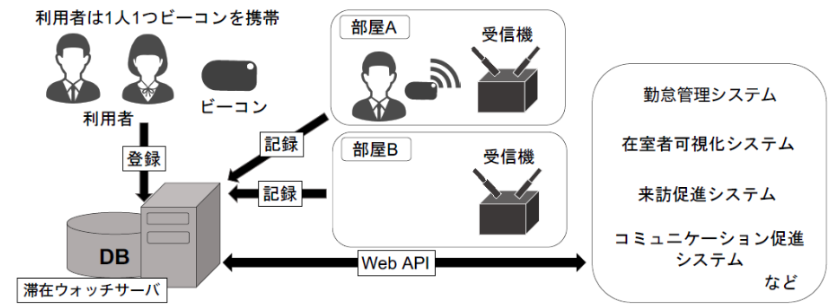
\includegraphics[width=8cm]{image/StayWatch.jpg}
  \caption{「滞在ウォッチ」の概要図}
  \label{multipleBPM}
\end{figure}

%--------------------------------------------





サーバ側には独立したバックエンドシステムとの連携を容易でありWebアプリケーションがバックエンドシステムとの親和性が高く、
より高い可用性とスケーラビリティを実現するができるREST APIを採用した.REST APIは、
複数のクライアントからアクセスができるため,様々なデバイスやプラットフォームからアクセスできる。これにより、より広いユーザー層からアクセスができる
既存の滞在ウォッチのサーバ側のシステムはpythonを用いて構築されており,動的型付け言語なため保守性が低いものであった.
そこで静的型付けであり,高速な処理能力と小さなメモリフットプリントを持つため、Web APIの開発に適しているGolangを採用した.
またGolangは並列処理を容易に実現できるため、高負荷な環境でのWeb APIの開発にも適している。さらに、標準パッケージによるHTTPサーバのサポートを持つため、
Web APIの開発に必要な機能を簡単に実装できる。
これらの特徴から、Golangを使用したWeb APIの開発は、高速でスケーラブルなAPIを提供することができ、開発効率も高い







サーバ側には独立したバックエンドシステムとの連携を容易でありWebアプリケーションがバックエンドシステムとの親和性が高く、
より高い可用性とスケーラビリティを実現するができるREST APIを採用した.REST APIは、
複数のクライアントからアクセスができるため,様々なデバイスやプラットフォームからアクセスできる。これにより、より広いユーザー層からアクセスができる
既存の滞在ウォッチのサーバ側のシステムはpythonを用いて構築されており,動的型付け言語なため保守性が低いものであった.
そこで静的型付けであり,高速な処理能力と小さなメモリフットプリントを持つため、Web APIの開発に適しているGolangを採用した.
またGolangは並列処理を容易に実現できるため、高負荷な環境でのWeb APIの開発にも適している。さらに、標準パッケージによるHTTPサーバのサポートを持つため、
Web APIの開発に必要な機能を簡単に実装できる。
これらの特徴から、Golangを使用したWeb APIの開発は、高速でスケーラブルなAPIを提供することができ、開発効率も高い

%--------------------------------------------

\section{今後の課題}
今後の課題として現段階では1つのコミュニティでの運用しかされていないため,実際に複数のコミュニティに導入してもらい,運用を行う必要がある.運用後は,ユーザからの意見や得られたデータを元にシステムの改善を行う予定である.また現状のシステムではコミュニケーションを促進するような仕組みがないためその仕組みづくりを行いたい.

%--------------------------------------------
\begin{thebibliography}{9}

  \bibitem{smartphone}\label{smartphone}
  嶋川司ら,
  スマートフォンとBLEビーコンを用いた出席管理手法の提案,
  THE HARRIS SCIENCE REVIEW OF DOSHISHA UNIVERSITY,VOL.58,No.2,2017.


  \bibitem{incom}\label{incom}
  中野利彦ら,
  Traveling Cafe: 分散型オフィス環境におけるコミュニケーション促進支援システム,
  インタラクション2006論文集,p227-228,2006.


\end{thebibliography}
\end{document}

%%% Local Variables: 
%%% mode: japanese-latex
%%% TeX-master: t
%%% End: 
